\documentclass[letterpaper, 12pt]{article}
\usepackage{geometry}
\usepackage{titling}
\usepackage{titlesec}
\usepackage{pgfplots}
\usepackage{tkz-euclide}
\usepackage{amsmath}
\usepackage{amsfonts}
\usepackage{amssymb}
\usepackage{amsthm}
\usepackage{bbold}
\usepackage{caption}
\usepackage{graphicx}
\usepackage{float}
\usepackage{mathtools}
\usepackage{bm}
\usepackage{titling}
\usepackage{fancyhdr}
\usepackage{bookmark}
\usepackage{fancyhdr}
\usepackage{tikz-cd}
\usepackage{hyperref}
\usepackage[utf8]{inputenc}
\usepackage[most]{tcolorbox} 
\usepackage[rightcaption]{sidecap}
\usepackage[shortlabels]{enumitem}


\renewcommand{\thesection}{\Roman{section}.}
\renewcommand{\thesubsection}{\null \quad \Alph{subsection}.}

\newcommand{\eqlabel}[1]{\label{eq:#1}}

% \hypersetup{hidelinks}
\geometry{margin=0.75in,top=1in}
\pgfplotsset{compat=1.18}


\titleformat{\section}[block]
  {\normalfont\normalsize\bfseries}
  {\thesection}
  {1em}{}

\titleformat{\subsection}[block]
  {\normalfont\normalsize\bfseries}
  {\thesubsection}
  {1em}{}


\begin{document}
   \setcounter{page}{0}.
    \begin{center}
        {\Large Simulating an Atomic Bomb - An Exercise in Neutron Diffusion\\}
        \vspace{0.5em}
        Evan Petrimoulx \\
    \end{center}

    \pagestyle{fancy}
    \fancyhf{}
    \fancyhead[R]{\today}
    \fancyhead[L]{Phys-3600 Computational Physics}
    \fancyfoot[R]{}
    \setlength{\droptitle}{-6em}

    \vspace{0.25cm}

    \tableofcontents
    \newpage
    \section{ Introduction}
      The aim of this project is to study the process of neutron diffusion and reaction inside of a reaction chamber. It will focus on how different materials such as U$^{235}$ and Pu$^{239}$ are used as fissile source materials for the reaction, and determine which materials are good choices to use as fuel sources. I will also investigate how the shape and size of these fuel rods affect the energy output of the system, and compare the energy output to items of similar scales such as heating a cup of water, or a nuclear weapons test. I will look at the minimum size of the fuel rod in order for a reaction to ensure, as well as investigate the scenario that gives the highest output possible. \\

      \begin{figure}[h!]
         \centering
         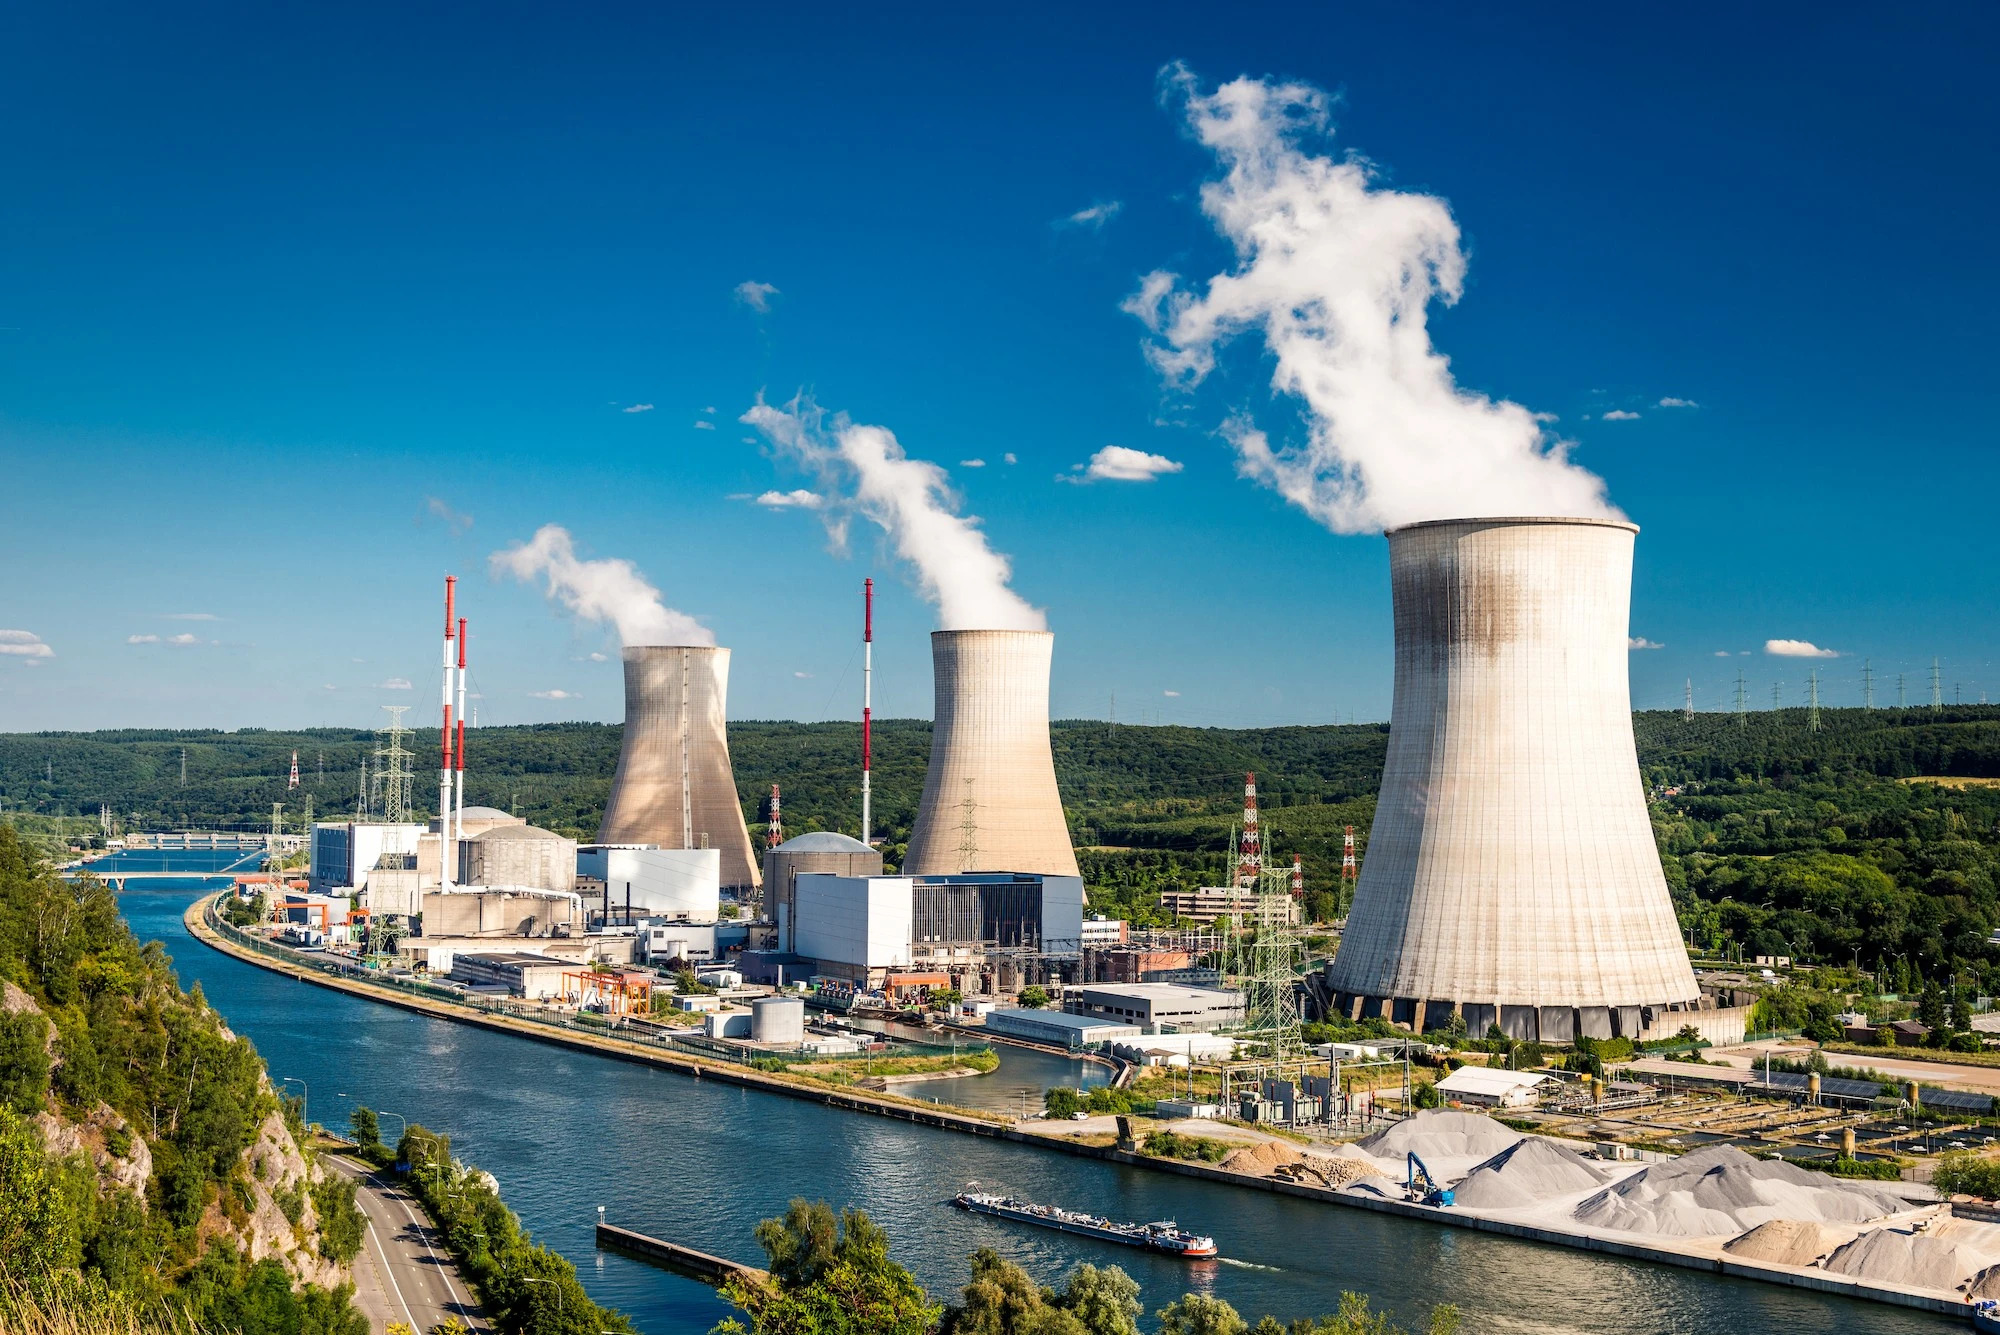
\includegraphics[width = 0.7\linewidth]{Images/Nuclear_Power_Plant.jpg}
         \caption{The above figure displays a nuclear power plant which uses fission as an energy source to supply electricity!}
         \label{img:Nuclear_Reactor}
      \end{figure}


      There are two common examples of this process; nuclear power plants \ref{img:Nuclear_Reactor} and atomic weapons of mass destruction \ref{img:Trinity_Test}. Nuclear power plants utilize the diffusion-reaction of fissile materials in a stable state, where the number of neutrons emitted from the reaction is a constant. This allows for control over the reaction, in which we can use the energy output to boil water, generate steam, and produce electricity. Atomic weapons utilize the diffusion-reaction of fissile materials in a super-critical state, where the reaction is so violent that there is an uncontrollable and exponential growth of produced neutrons, emitting vast amounts of energy in a large explosion. These types of weapons are what was used at the end of the second World War by the Americans to conclude the war in the Pacific. \\

      This report will focus primarily on unstable, exponentially growing production of neutrons, and will investigate various configurations of interacting fissile material, comparing its energy output to items of similar scale. I will also discuss energy output optimization, and how to determine the largest output energy possible given two sources of fissile material. Determining the best material to use for the diffusion process, as well as determining the distance of separation between the two objects and their minimum possible size to produce a reaction will also be areas of investigation within this report.

    \section{ Background}
      \subsection{What is Diffusion?}
         Diffusion is defined as "the spreading of something more widely". It can be described as the movement of particles from an area of high concentration to an area of low concentration until an equilibrium is reached \cite{Diffusion-Defn}. It is responsible for the way a smell from your kitchen travels around your house, how your body processes and breathes in Oxygen into your lungs, how the mist from a perfume bottle spreads outwards, and even how your car warms up when you turn the engine on. Diffusion is present in almost everything we do, and has many practical applications in science and engineering. \textit{Neutron Diffusion} is the process in which neutrons from some source are ejected from their nucleus and disperse throughout a medium. It is commonly used in nuclear reactors to produce energy. 

      \subsection{History}
         The phenomena of diffusion has been known since the early 19th century. The work was primarily discovered by Jean Baptiste Joseph Fourier in 1807, where he presented his formula for the dispersion of heat throughout a solid. It wasn't until he published his work on \textit{The Analytic Theory of Heat} in 1822 when his theories of heat had finally become accepted by scientists \cite{History}. His equation for the diffusion of heat can be written down as the following partial differential equation:

         \begin{equation}
            \frac{\partial}{\partial t} \phi (\vec{r}, t) = \kappa \nabla^2 \phi (\vec{r}, t)
         \end{equation}

         If this equation is constrained to the initial conditions that the Heat at the boundaries is zero, known as \textit{Dirichlet boundary conditions}, and the Heat at the initial time is given by some function, we can show that the PDE has the following solution for a rectangular prism of width $a$, length $b$, and height $c$:

         \begin{equation}
            \phi (\vec{r}, t) = \frac{8}{abc} \sum_{m=1}^\infty \sum_{n=1}^\infty \sum_{l = 1}^\infty  A_{mnl} \sin \left( \frac{m \pi x}{a} \right) \sin \left( \frac{n \pi y}{b} \right) \sin \left( \frac{l \pi z}{c} \right) e^{-\kappa \pi^2 \left( \frac{m^2}{a^2} + \frac{n^2}{b^2} + \frac{l^2}{c^2}\right) t}
         \end{equation}

         Where $ A_{mnl}$ is defined as:

         \begin{equation}
            A_{mnl} = \int_0^a \int_0^b \int_0^c \phi (\vec{r}, 0) \sin \left( \frac{m \pi x}{a} \right) \sin \left( \frac{n \pi y}{b} \right) \sin \left( \frac{l \pi z}{c} \right)dx dy dz
         \end{equation}

         Since the equation is a PDE, its solution can have multiple forms depending on the shape of the object, and the boundary conditions being applied. It behaves as a decaying exponential, which implies that when the boundaries absorb heat, the material will eventually radiate all of its heat away and return back to equillibrium. This equation was not as "obvious" as it might seem to us, since there was no guarentee that the right hand side of the equation converged. It took Fourier more than 50 years to prove the convergence with his discovery of the \textit{Fourier Series} \cite{History}. The heat equation is now considered a cornerstone of the theory of thermodynamics and is well studied by students in Physics and Engineering.\\

         Fast forwarding through time, we now get to the 20th century. The discovery of Quantum Mechanics has revolutionized the worlds understanding of Physics, and while it was a great time of growth for science, it was also a time of war. Scientists had just discovered that it was possible to split an atom, and unleashing the strong force became of great interest due to the high amounts of energy this process could release. Countries on both the Allied and Axis forces scrambled to find a way to make a weapon they could unleash on their enemies and stop the war in its tracks. Scientists at Los Alamos found that by using fissile materials such as Plutonium-239, they could initiate a diffusion-reaction of neutrons by splitting the nucleus of the atom apart. This process would fire off neutrons which would then collide and interact with other neutrons, creating even more neutrons, releasing even more energy. This cycle would continue until the sources were annihilated, and a violent explosion from the release of energy would ensue \ref{img:Trinity_Test}. The equation that modelled this process is known as the \textit{Diffusion-Reaction Equation}. The scientists at Los Alamos were able to successfully create the worlds first atomic bomb before the Nazis, and the first bomb was set off in a test known as \textit{Trinity} on July 16th 1945. The United States used their remaining two atomic warheads to end the war in the Pacific, forcing a surrender from the Japanese forces in just three days.\\

         \begin{figure}
            \centering
            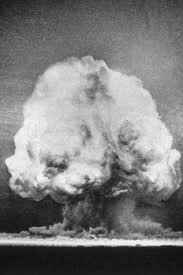
\includegraphics[width = 0.25\linewidth]{Images/Trinity_Test.jpg}
            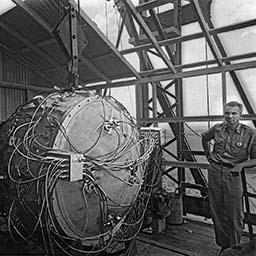
\includegraphics[width = 0.3763\linewidth]{Images/Trinity_Bomb.jpg}
            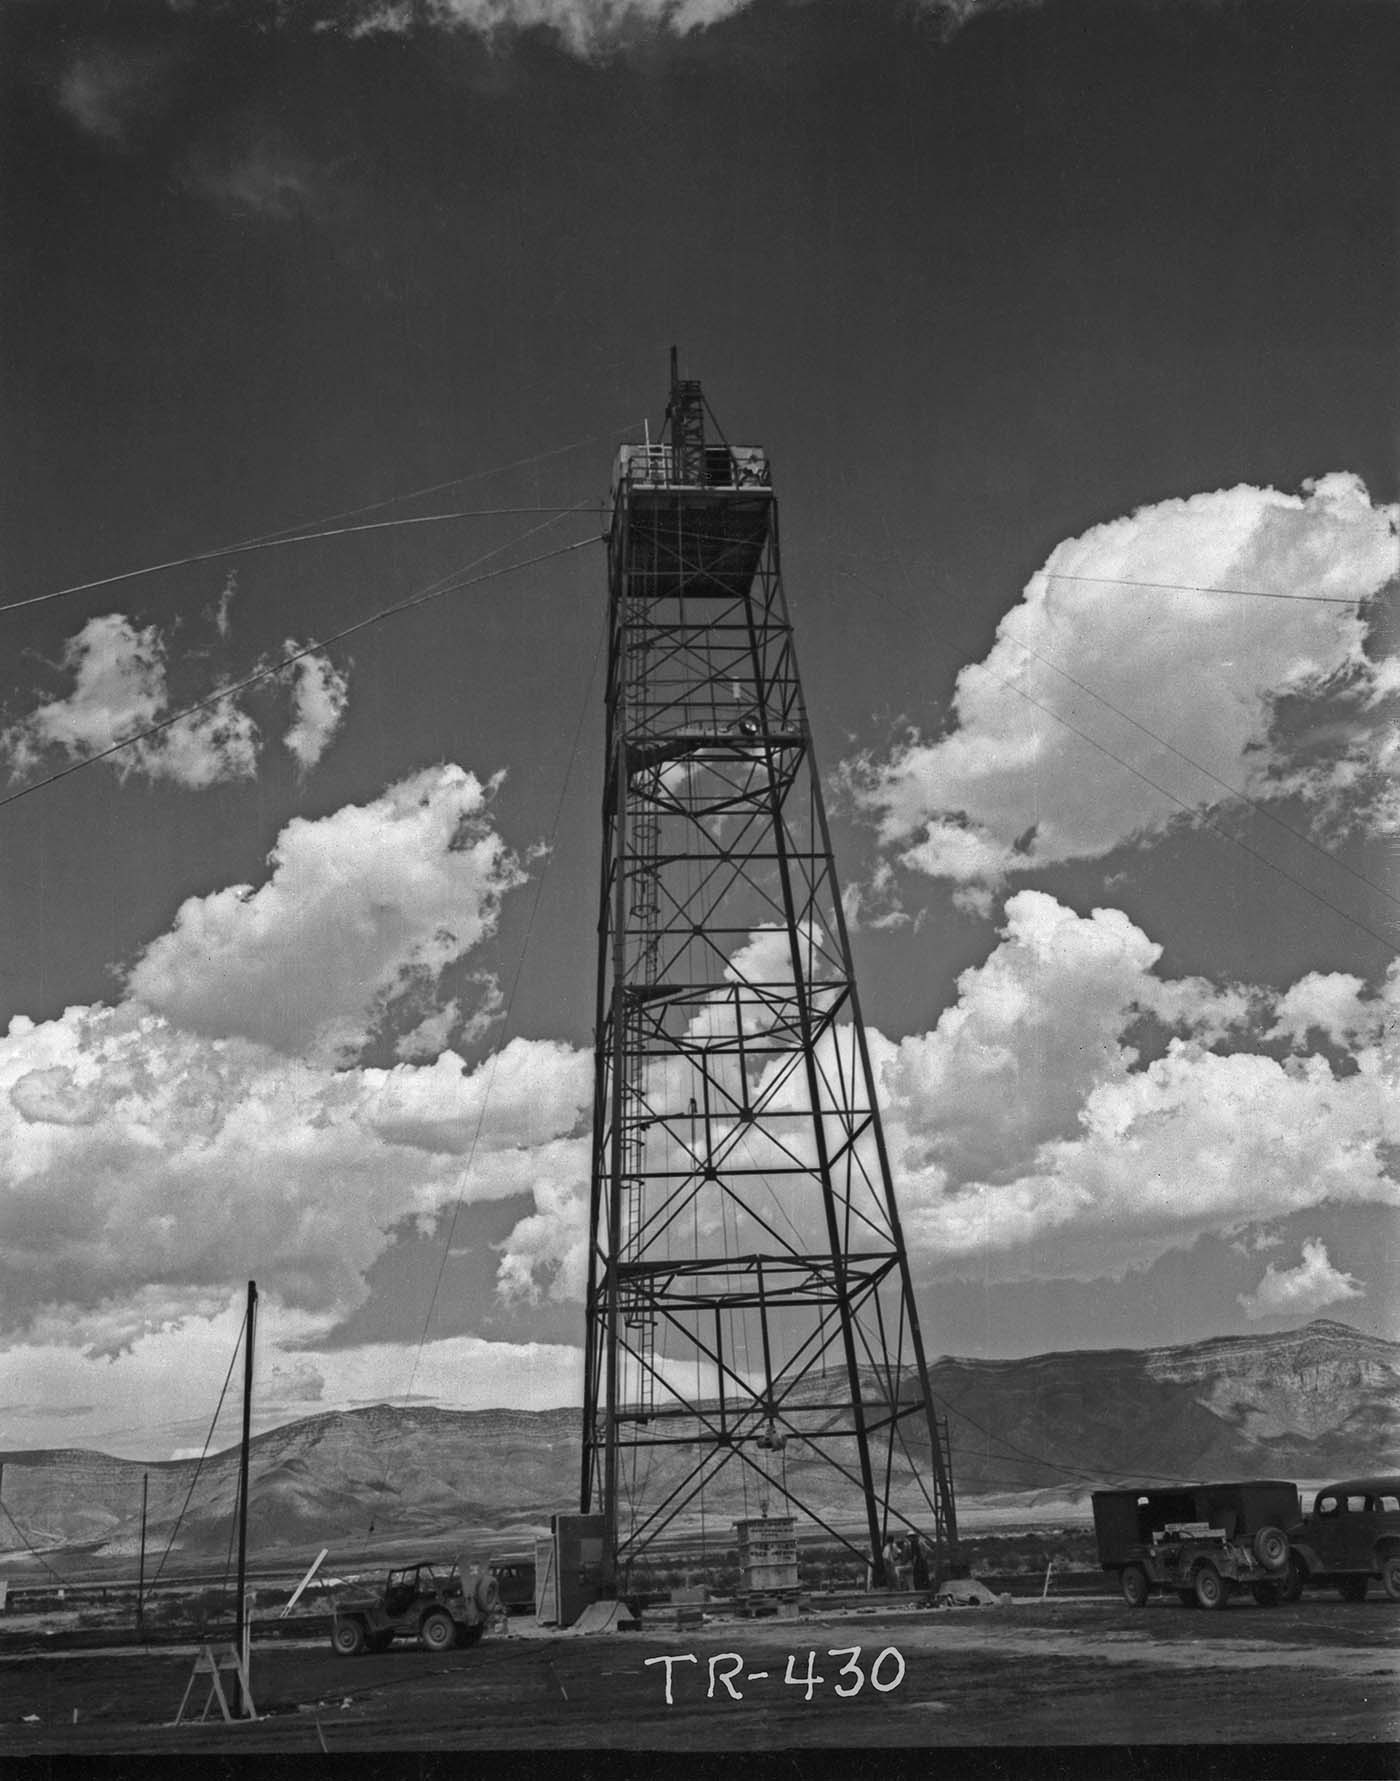
\includegraphics[width = 0.294\linewidth]{Images/Trinity_Tower.jpg}
            \caption{The Detonation of the first atomic bomb, named Trinity, on July 16th 1945 in Los Alamos, New Mexico, USA}
            \label{img:Trinity_Test}
         \end{figure}

         Fast forwarding to the present, the world has utilized the discovery for good, and scientists learned how to handle the reaction in a stable and managable state. Nuclear power plants have been constructed which are capable of powering entire cities with just a few kilograms of Uranium, and the diffusion process is studied by many nuclear engineers and physicists who research how to harness the energy released from the reaction.

      \subsection{The Diffusion-Reaction Equation}
         Diffusion is a process in which something moves from an area of high density to an area of lower density. It can be described in physical systems by \textit{Fick's equation} \cite{Nuclear_Power_2021}. This one dimensional equation is analgous to the heat equation, where the right hand side handles the dispersion of material over space, and then left hand side describes the dispersion of material over time. 

         \begin{align*}
            J = -D \frac{\partial n}{\partial x}
         \end{align*}

         Here, $D$ is the diffusion coefficient, $J$ is the diffusion flux (The amount of material moving away from the region of higher concentration per unit area per unit time), $n$ is the concentration of the material and $x$ is its position. Differentiating both sides of the equation with respect to position we retrieve the heat equation.\\

         In a diffusion-reaction process, the material that is diffusing away from the source also interacts with its surroundings. Neutrons that are fired off from the nucleus can collide with other particles to create \textit{more} neutrons. The diffusion reaction equation is modelled as an extension to Fick's equation and the heat equation, and is written as:

         \begin{equation}
            \frac{\partial}{\partial t} \phi (\vec{r}, t) = \kappa \nabla^2 \phi (\vec{r}, t) + \eta \phi (\vec{r}, t)
         \end{equation}

         Where $\eta$ is the reaction rate of the system, and describes how the neutrons interact with their environment to either absorb or create more fission. The greater the value of $\eta$, the more fission occurs, and the density and energy output increases. If the reaction rate is negative, it means more neutrons are being absorbed than generated, and the system's density decreases.
    \section{ Neutron Diffusion Reaction}
      In this section we will model the diffusion-reaction equation in 3D space using 2 fuel rods as neutron sources. The simulation grid is set to a 40 meter wide cube, and the fuel rods are placed inside of the 3D mesh. The diffusion-reaction equation is modelled numerically using a 3D stencil and a finite difference method solver for the spatial derivatives.

      \begin{equation}
         \nabla^2 n \approx \frac{1}{\delta x^2} \left( n_{i+1, j, k} + n_{i-1, j, k} + n_{i, j+1, k} + n_{i, j-1, k} + n_{i, j, k+1} + n_{i, j, k-1} - 6n_{i, j, k} \right).
      \end{equation}

      \begin{figure}[h!]
         \centering
         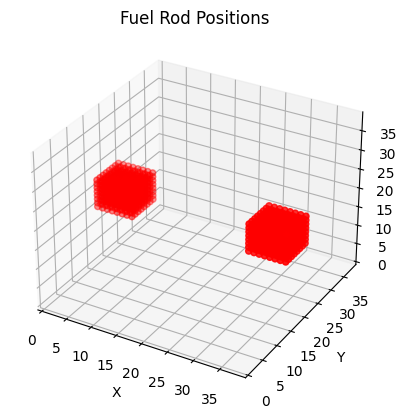
\includegraphics[width=0.4\linewidth]{Graphs/Graph_FuelRodsInGrid.png}
         \caption{Image of two cube-shaped fuel rods being placed into the simulation grid.}
      \end{figure}

      \subsection{Choosing a material}
         Since neutron-reactions are of key interest for energy production, whether it be stable and controlled energy release or rapid and destructive, the best choice of material stays the same. In order to get the highest energy output, you want to choose a material where the diffusion constant $D$ and the reaction constant $\eta$, are very large. The diffusion constant controls how much material per unit area is diffusing or moving away from the source per second. The higher the flux of the neutrons, the more energy you can harness from them. The reaction rate term controls the multiplying factor of the emitted neutrons. The higher the multiplication factor, the more neutrons are likely to be created during the reaction.\\

         The diffusion constant can be determined via a simple relation with the neutron's speed ($v_{\text{neut}}$) and its transport free path $\lambda_t$ \cite{Griffiths_2020}:
         \begin{equation}
            D = \frac{\lambda_t v_{\text{neut}}}{3}
         \end{equation}

         And similarly, the reaction rate $\eta$ can be determined with the neutron's speed, the \textit{fission} free path $\lambda_f$ and the secondary created neutrons from the fission process. It is described mathematically below:
         \begin{equation}
            \eta = \frac{v_{\text{neut}} \left( \nu - 1 \right)}{\lambda_f}
         \end{equation}

         Where the minus one accounts for the neutron that is consumed in the fission reaction. These values can be determined using known properties of elements, but in this report, we rely on table 7 from Griffiths' calculation \cite{Griffiths_2020}. In his paper, Griffiths gives a reaction rate for U$^{235}$ as $2.345 \times 10^5 m^2/s$, and a reaction rate $\eta = 1.896 \times 10^{8} s^{-1}$. For $Pu^{239}$, the reference gives $D = 2.678 \times 10^{5} m^2/s$ and $\eta = 3.005 \times 10^8 s^{-1}$. We can see that both materials have a very large reaction rate and diffusion constant, which make them excellent choices for neutron fuel sources.\\

         \begin{figure}
            \centering
            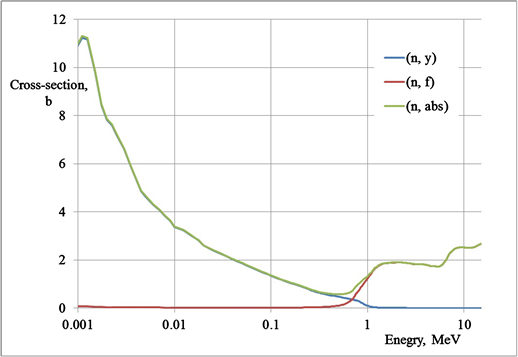
\includegraphics[width=0.5\linewidth]{Graphs/Americium-Graph.png}
            \caption{Image of the diffusion constant and absorption constant related to the elements energy in MeV. This graph was obtained from \cite{article}. (n, abs) is the absorption coefficient, and (n, f) is the fission or diffusion constant.}
            \label{Americium}
         \end{figure}

         The choice of these materials is carefully chosen, based on these two factors. While it is true that larger nuclei require much less energy to break apart, the reason that we do not use even larger elements such as Americium is because they have larger absorption cross sections than their fission cross section. This means that their reactions are almost always sub-critical because the amount of neutrons absorbed is much greater than that in which they are able to produce during fission \cite{article} It just so happens that Uranium and Plutonium isotopes do not have this feature, and their fission cross section is much larger than their absorption. We do not have an interest in using smaller atoms such as iron either, since they are extremely stable on their own, and require more energy to break apart than they release. According to K. Hirano, M. Cohen, and B.L. Averbach, the diffusion constant of paramagnetic alpha iron above $800^\circ C$ is only $1.3 \exp(-56000 / RT)$ \cite{Hirano_Cohen_Averbach_1961}, where $R$ is the universal gas constant, and T is the absolute temperature in Kelvin \cite{6.2.3.1_2013}. The $RT$ term represents the average kinetic energy of the material. If we use $800^\circ C$ as our starting point we see that the diffusion constant in paramagnetic alpha iron is:

         \begin{align}
            D = 1.3\exp \left(\frac{-56000}{ 8.314 \text{ J/mol } 1073.15 \text{K}}\right) \longrightarrow D = 0.0024 m^2/s
         \end{align}

         So we definitely do not want to use Iron in our reaction! It would require us to heat up the iron to more than $800^\circ C$ before there was even the smallest amount of diffusion, that the energy consumed is much more than that produced. \\

         Comparing between the two main choices of Uranium-235 and Plutonium-239, Plutonium-239 is clearly the better choice. However, taking into consideration the difficulty in producing enriched Plutonium, Uranium-235 is easier to obtain in larger quantities, and is more commonly used in the United States \cite{What-is-Plutonium?}.
      \subsection{Small scale diffusion-reaction}
         How small can we make the objects such that they don't diffuse at all anymore? To determine this, I had to adjust the setup of my implementation. As a default, the program implements the simulation in SI units, this means the objects size is initialized in meters. To adjust for this, I applied a conversion factor when applying the initial conditions from cubic meters to cubic millimeters, and set up the fuel rods to be points in space. Since the fuel rod grid is in meters, anything smaller than a 1m$^3$ shape will appear as a point. So the smaller scale simulations behave as point sources with a smaller density to match that of an equivalent 1mm cube of Plutonium-239. 

         \begin{figure}[h!]
            \centering
            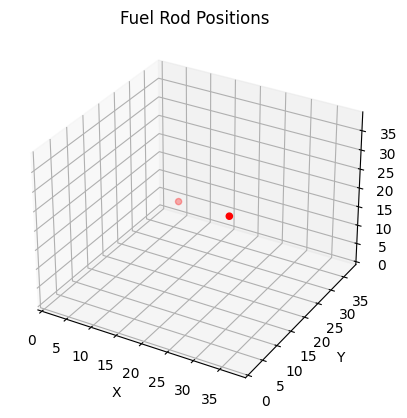
\includegraphics[width=0.4\linewidth]{Graphs/Small-Simulation.png}
            \caption{Image of 2 point source neutron emitters placed in the grid.}
            \label{img:Small Objects in Grid}
         \end{figure}

         \begin{figure}[h!]
            \centering
            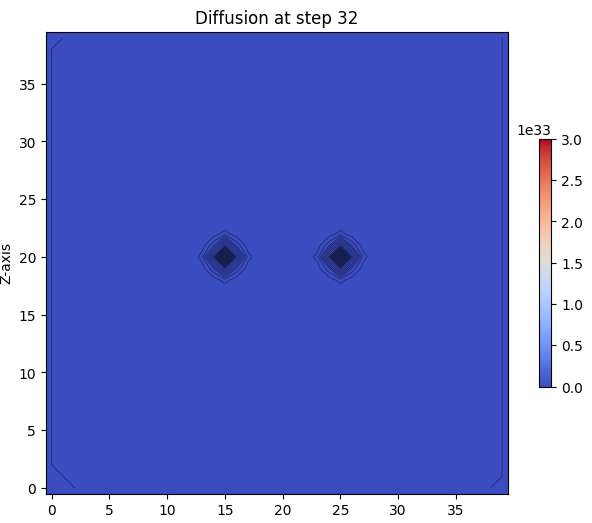
\includegraphics[width=0.23\linewidth]{Images/Small-Source-1.png}
            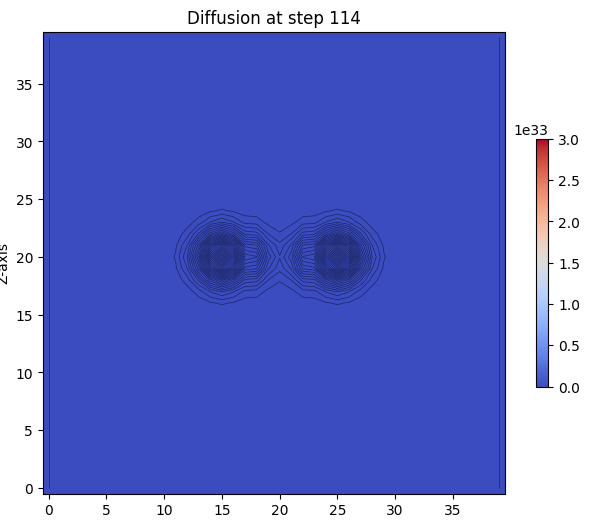
\includegraphics[width=0.23\linewidth]{Images/Small-Source-2.png}
            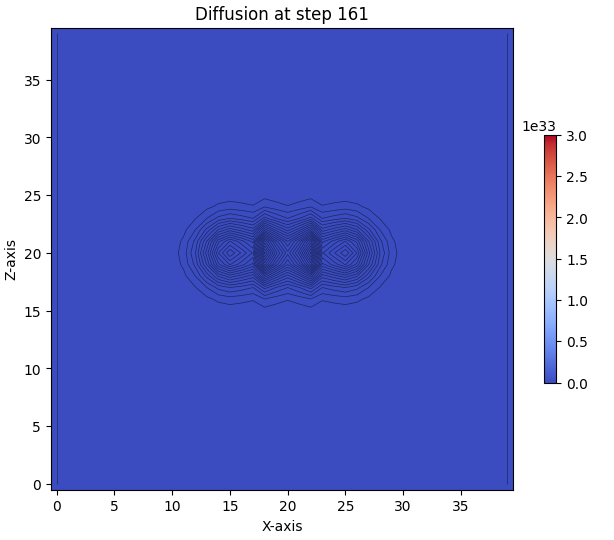
\includegraphics[width=0.23\linewidth]{Images/Small-Source-3.png}
            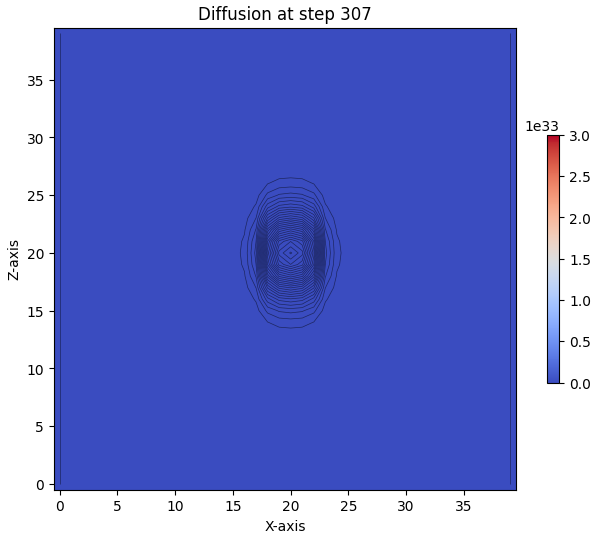
\includegraphics[width=0.23\linewidth]{Images/Small-Source-4.png}
            \caption{Images of diffusion of the small diffusion of two 1mm Plutonium Cubes.}
            \label{img:1mm-Plutonium}
         \end{figure}

         
         According to the simulation, this object does produce neutrons! However, only an extremely small amount. Calculating the energy from the density of neutrons at the beginning and the end of the simulation with equation \ref{eq:Energy} we can see that $5420$ J are released!
         
         \begin{equation}
            E = \rho V \cdot 2 \frac{\text{MeV}}{\text{neutron}} \cdot 1.6022 \times 10^{-13} \frac{\text{MeV}}{\text{J}}
            \eqlabel{Energy}
         \end{equation}
         
         To put this into perspective, we can use the heat equation from Chemistry shown by equation \ref{eq:Chemistry} for a specific heat of water of $c = 4184 J/kg ^\circ C$ and a volume of $250$mL to show that this energy release is equivalent to heating up a $250$mL cup of water by $5.64^\circ C$. This is not a lot of energy, and is roughly in a stable state, so I will consider this reaction non-super-critical, since the output of energy really isnt high enough to be meaningful and likely would be absorbed or lost during the process of starting the diffusion anyways. 

         \begin{equation}
            Q = mc \Delta T \longrightarrow \Delta T = \frac{Q}{mc}
            \eqlabel{Chemistry}
         \end{equation}

         Making the fuel rods a bit larger, I can calculate the energy release for two 1cm cubes. 

         \begin{figure}
            \centering
            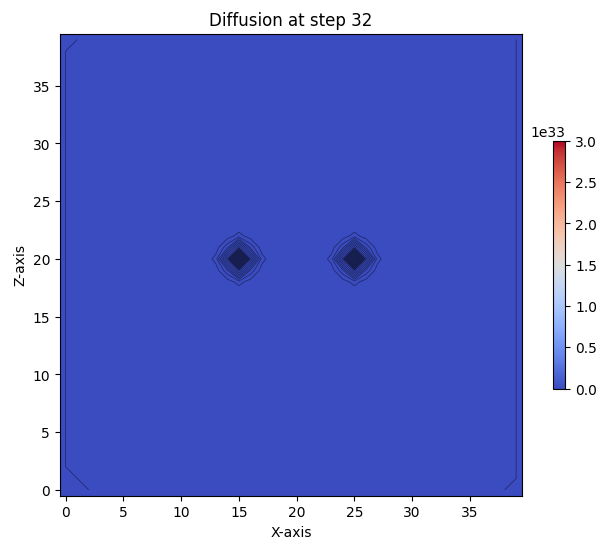
\includegraphics[width=0.23\linewidth]{Images/1cm-Source-1.png}
            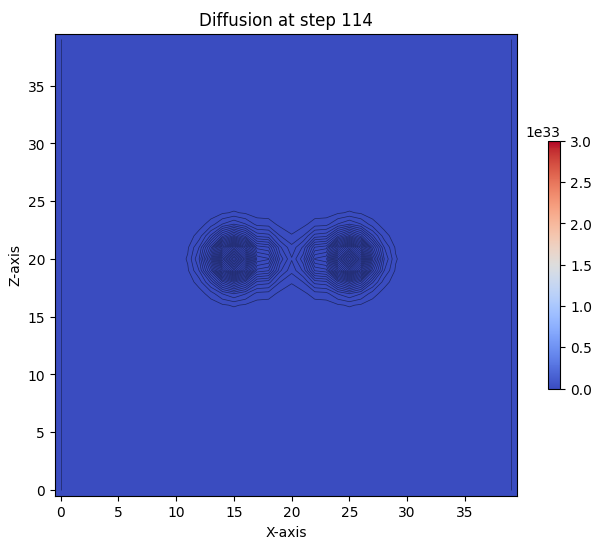
\includegraphics[width=0.23\linewidth]{Images/1cm-Source-2.png}
            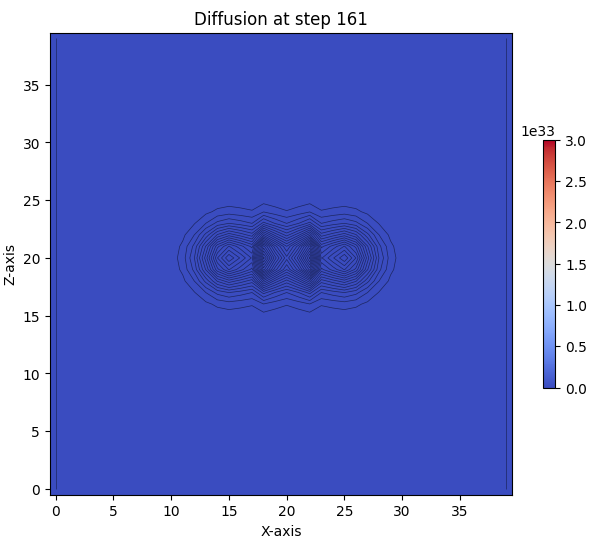
\includegraphics[width=0.23\linewidth]{Images/1cm-Source-3.png}
            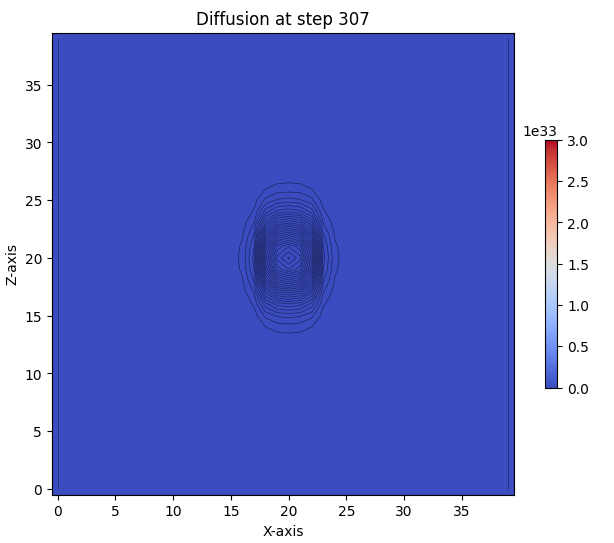
\includegraphics[width=0.23\linewidth]{Images/1cm-Source-4.png}
            \caption{Images of diffusion of the small diffusion of two 1cm Plutonium Cubes.}
            \label{img:1cm-Plutonium}
         \end{figure}

         As shown in figure \ref{img:1cm-Plutonium} we can see that the number of neutrons is growing. This is highlighted better in the neutron density over time graph shown in figure \ref{img:1cm-Plutonium-Graph}. We can see here that fission is occurring in the simulation and energy is being emitted. Calculating the energy release again with equation \eqref{eq:Energy} we calculate that this time, $5.88 \times 10^6$ J are released. Comparing this with equation \eqref{eq:Chemistry} like we did for the 1mm cubes, we can see that this is equivalent to heating up a 250mL cup of water by $5619.6^\circ C$! This is too high to be a reasonable comparison, so lets move on to a comparison that is a little bit more fun.\\

         Explosions are measured in terms of kilograms of TNT. Shown below is a formula we can use to relate the amount of energy in Joules released, to the amount of TNT the explosion is equivalent to:

         \begin{equation}
            \frac{E}{4.184 \times 10^9 \text{J/ton of TNT}} = \text{tons of TNT}
            \eqlabel{Tons-of-TNT}
         \end{equation}

         Using this formula \eqref{eq:Tons-of-TNT} with our  $5.88 \times 10^6$ J of released energy, we find that using 2 cubes of Plutonium-239 that have length of 1cm is equivalent to the explosive power of $1.4 \times 10^{-3}$ tons of TNT. Equivalently, this is $1.4$kg of TNT. So we have made a small explosion, but nothing that will be anywheres close to the orders of magnitude of a traditional nuclear weapon. So while the fission process is possible for even 1 Uranium atom theoretically, we can safely say that unless you have around two 1cm by 1cm by 1cm cubes of Uranium, nothing meaningful will happen on a human scale, unless you want to heat up your cup of coffee.

         \begin{figure}[b!]
            \centering
            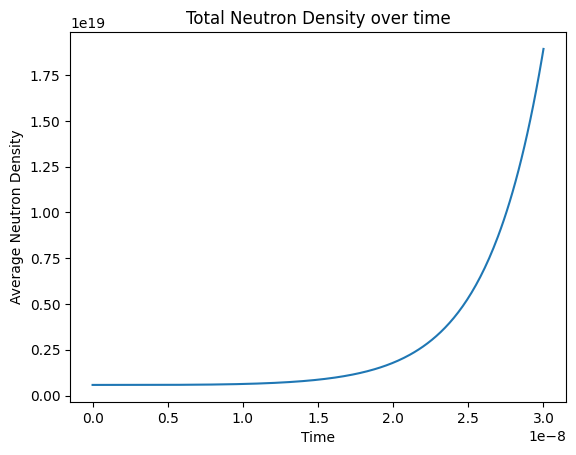
\includegraphics[width=0.4\linewidth]{Graphs/1cm-Cube.png}
            \caption{Graph depicting the average number of neutrons over time for two 1cm cubes. Notice that the growth is still exponential, but the total density is still several orders of magnitude lower than the usual simulations.}
            \label{img:1cm-Plutonium-Graph}
         \end{figure}

      \subsection{The effects of fuel rod shape on the energy output}
         In this section I will investigate how the shapes of the fuel rods can affect the energy output. I will be mainly utilizing equation \eqref{eq:Tons-of-TNT} to make these comparisons and relate the output to known values. We can expect the energy output of these systems to be much larger than normal reactions however, since our fuel rods are significantly bigger than any reactor constructed before. In order to help with the comparison, I will compare the output to the explosions of the TSAR Bomba, the largest nuclear warhead ever detonated in human history.\\

         The TSAR Bomba was a thermonuclear aerial bomb developed and tested by the Soviets in 1961. The explosion is estimated to have yielded around 58 Mega-Tons of TNT, or around 243 PJ. If the weapon had a slightly larger deposit of Uranium in the warhead, it was predicted to have been capable of releaseing over 100 Mega-Tons of TNT, or around 418 PJ. The Uranium deposit was lessened in order to reduce the amount of fallout radiation from the explosion \cite{TSAR-BOMBA}.\\

         So far we have analyzed the energy output of 2 Cubes of Uranium-235 and Plutonium-239. For this segment we will investigate the dependance of shape of fuel rods on the energy output of the system for Uranium fuel rods only. This is just to keep the numbers a bit more reasonable since the scale of our simulation is very large. We can create the Uranium Fuel rods using an object class, and calculate their volumes and neutron densities before placing them into the simulation grid. To do so, we just fill a 3D box with neutrons in the desired shape. This doesn't give us a perfectly accurate shape, but increasing the size of the box as well as the spatial step in the simulation can lead to more accurate shape construction. We will start with the case of a sphere and a hemisphere colliding, as depicted in figure \ref{img:Sphere-and-Hemisphere}.\\

         Analyzing the images of the neutron density over time for the far apart fuel rods (20m separation) as well as the images of the neutron density for the rods that are close together (8m separation) \ref{img:Sphere-and-hemisphere-density}, we can see that the energy production increases dramatically as the separation decreases. Calculating the energy release with equation \eqref{eq:Energy} we can see that the energy emitted from the reaction of the two spherical and hemispherical rods releases $1.11 \times 10^{13}$ J, and when brought closer together to the 8m separation distance, emit $5.41 \times 10^{17}$ J. This is equivalent to 129 Million tons of TNT, or about the size of 2 TSAR Bombas. 

         \begin{figure}
            \centering
            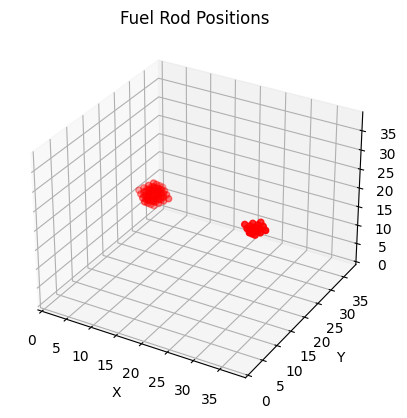
\includegraphics[width=0.4\linewidth]{Graphs/Sphere-and-Hemisphere-Far.png}
            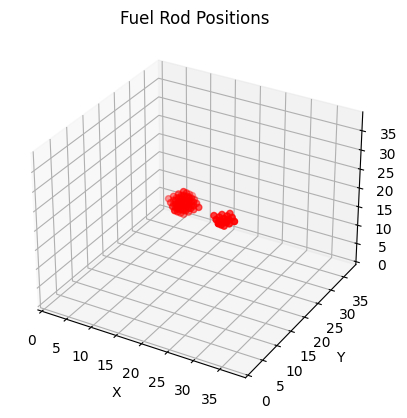
\includegraphics[width=0.4\linewidth]{Graphs/Sphere-and-Hemisphere-Close.png}
            \caption{Image of Colliding spherical fuel rod and hemisphericalfuel rod in the simulation grid.}
            \label{img:Sphere-and-Hemisphere}
         \end{figure}

         \begin{figure}
            \centering
            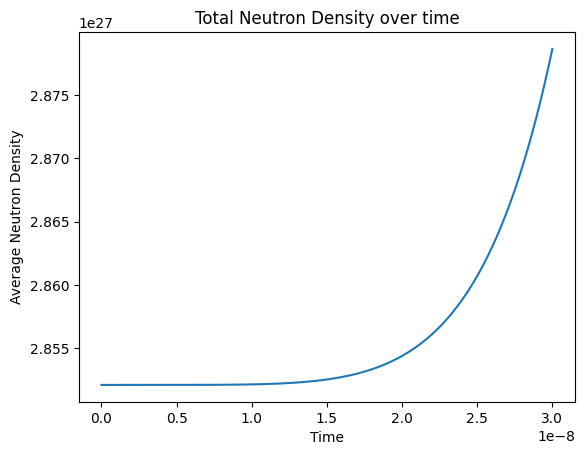
\includegraphics[width=0.4\linewidth]{Graphs/Sphere-and-Hemisphere-Far-Density.png}
            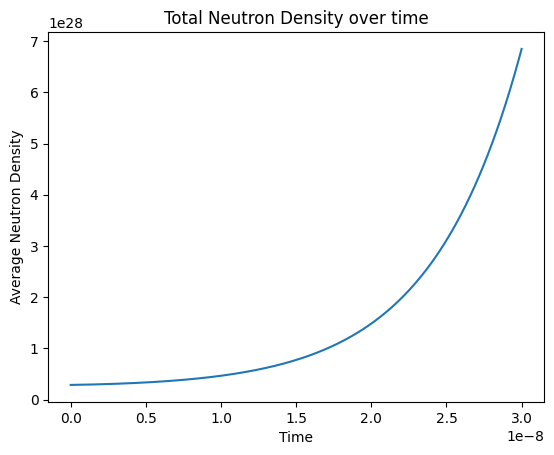
\includegraphics[width=0.4\linewidth]{Graphs/Sphere-and-Hemisphere-Close-Density.png}
            \caption{Image of neutron density over time for the spherical and hemisphereical fuel rods.}
            \label{img:Sphere-and-hemisphere-density}
         \end{figure}

         \begin{figure}[h!]
            \centering
            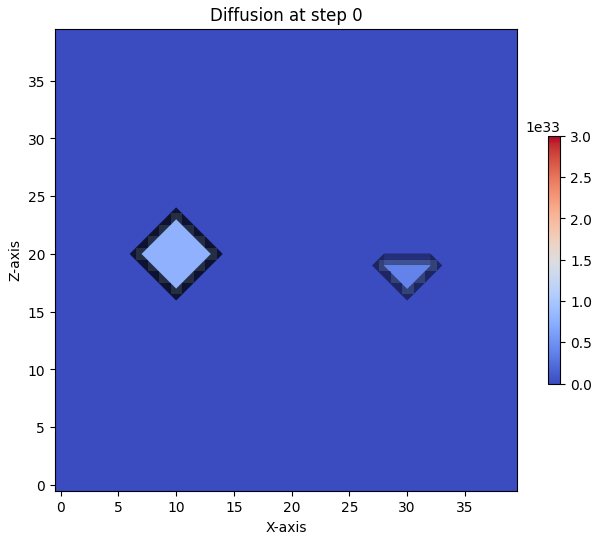
\includegraphics[width=0.22\linewidth]{Images/Sphere-and-Hemisphere-Far-1.png}
            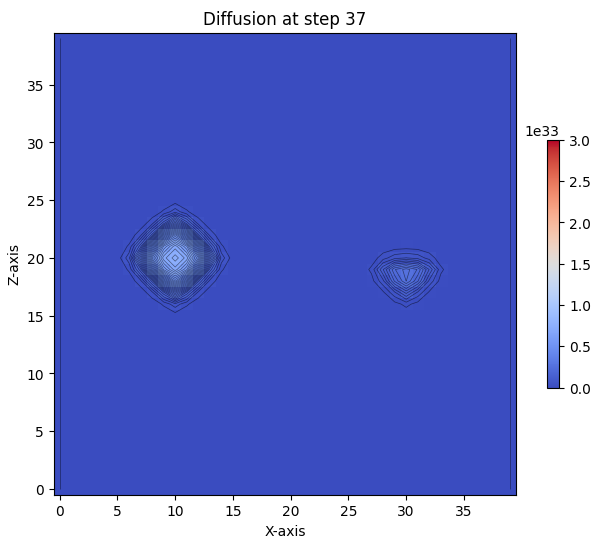
\includegraphics[width=0.22\linewidth]{Images/Sphere-and-Hemisphere-Far-2.png}
            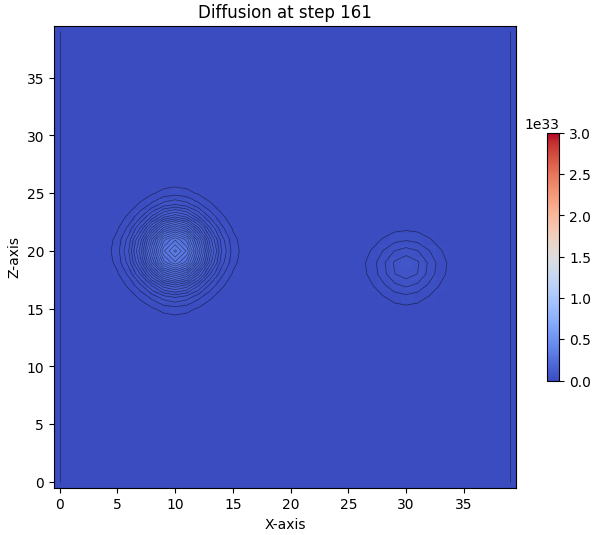
\includegraphics[width=0.22\linewidth]{Images/Sphere-and-Hemisphere-Far-3.png}
            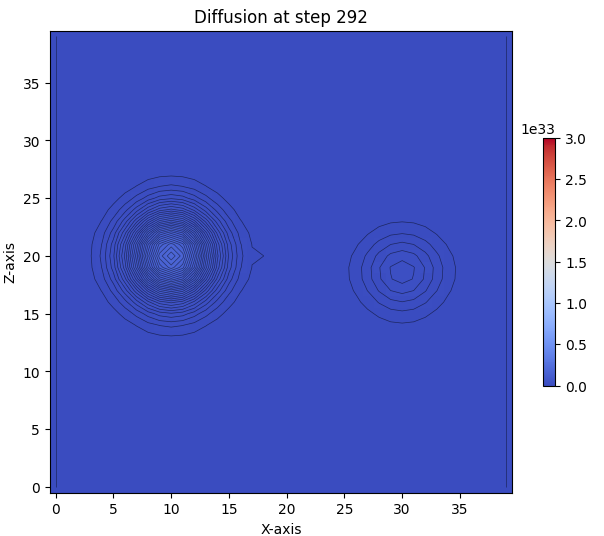
\includegraphics[width=0.22\linewidth]{Images/Sphere-and-Hemisphere-Far-4.png}\\
            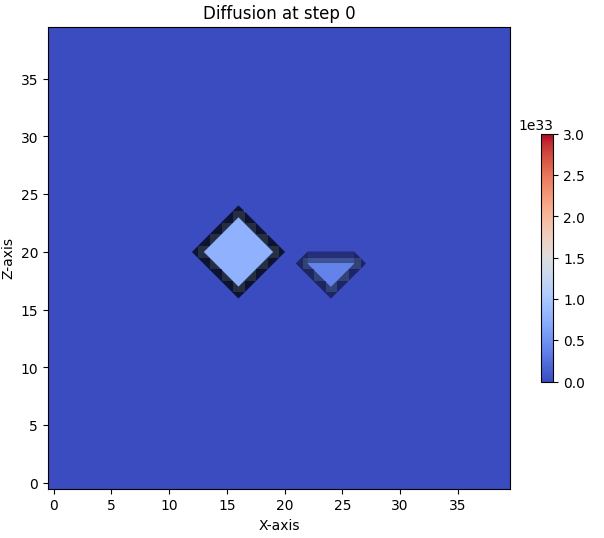
\includegraphics[width=0.22\linewidth]{Images/Sphere-and-Hemisphere-Close-1.png}
            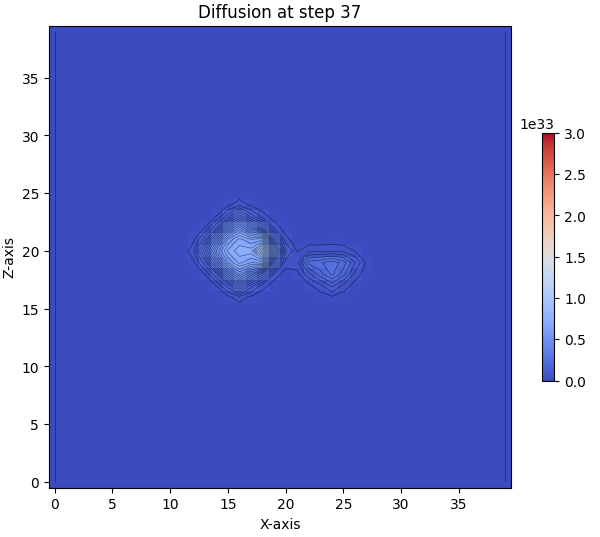
\includegraphics[width=0.22\linewidth]{Images/Sphere-and-Hemisphere-Close-2.png}
            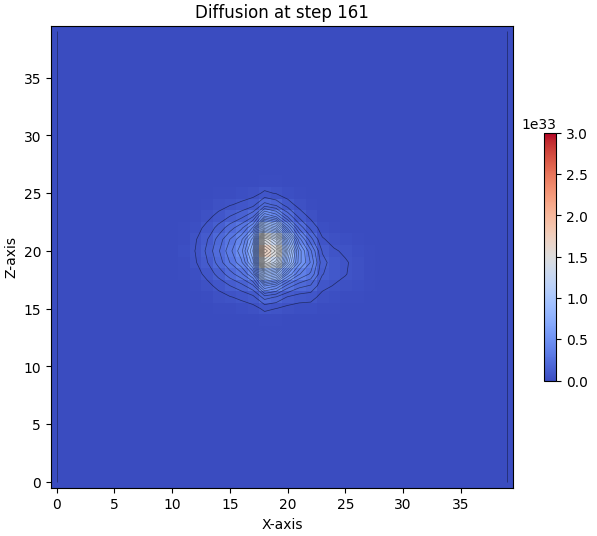
\includegraphics[width=0.22\linewidth]{Images/Sphere-and-Hemisphere-Close-3.png}
            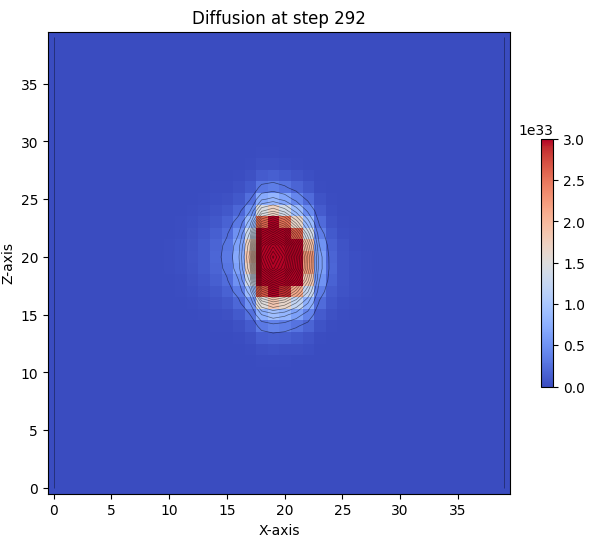
\includegraphics[width=0.22\linewidth]{Images/Sphere-and-Hemisphere-Close-4.png}
            \caption{Image of spatial distribution of neutron density for the Spherical and Hemi-Spherical rods. The distribution of neutron density for the 20m separation (Top) and the distribution of neutron density for the 8m separation (below)}
            \label{img:Sphere-and-hemisphere-images}
         \end{figure}

         I will test one more combination of shapes, considering a Triangular prism and a cylinder interacting with one another. There are several combinations to be tested here, but to keep this sectino short and not clutter the report with images, the 2 cases other than the colliding cubes will be the only discussed here. For more combinations to test, refer to the code written within the submitted Jupyter Notebook. \\

         \begin{figure}[h!]
            \centering
            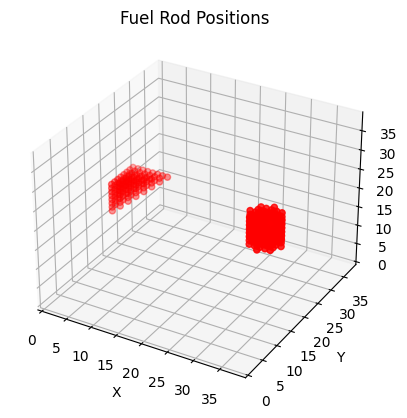
\includegraphics[width=0.4\linewidth]{Graphs/Cylinder-Prism-Far-Grid.png}
            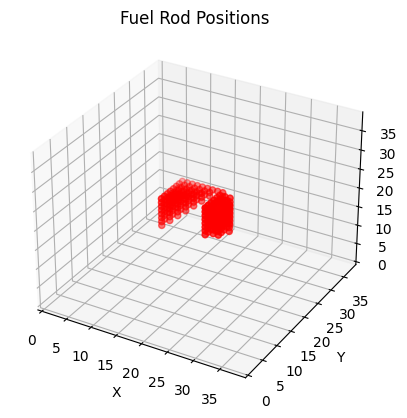
\includegraphics[width=0.4\linewidth]{Graphs/Cylinder-Prism-Close-Grid.png}
            \caption{Image of Colliding Triangular Prism and Cylindrical shaped fuel rod in the simulation grid.}
            \label{img:Prism-and-Cylinder}
         \end{figure}

         \begin{figure}[b!]
            \centering
            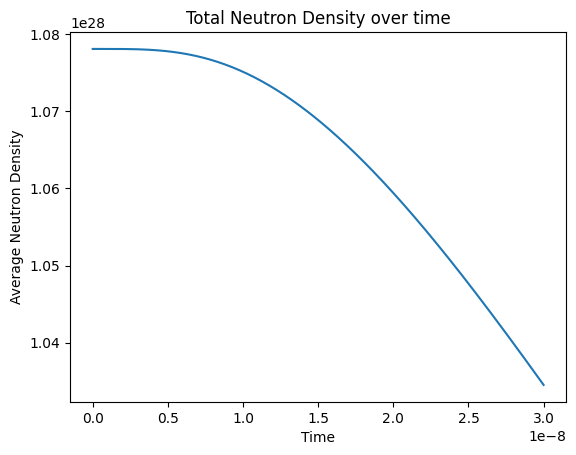
\includegraphics[width=0.4\linewidth]{Graphs/Cylinder-Prism-Far-Graph.png}
            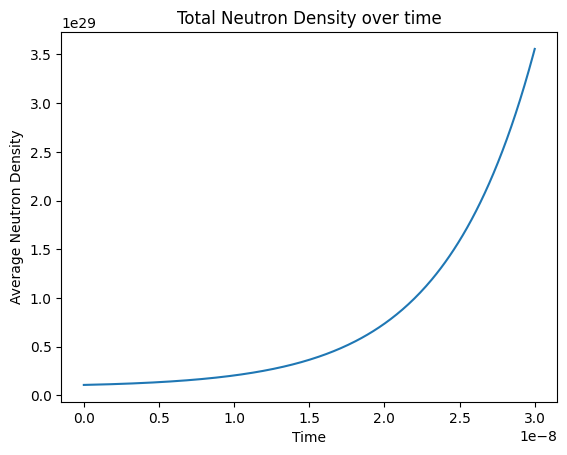
\includegraphics[width=0.4\linewidth]{Graphs/Cylinder-Prism-Close-Graph.png}
            \caption{Image of neutron density over time for the Triangular Prism and Cylindrical fuel rods.}
            \label{img:Prism-and-Cylinder-density}
         \end{figure}

         \begin{figure}
            \centering
            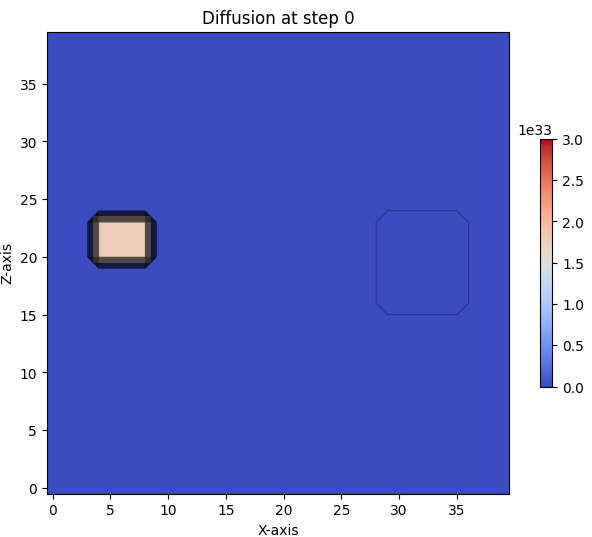
\includegraphics[width=0.22\linewidth]{Images/Cylinder-Prism-Far-1.png}
            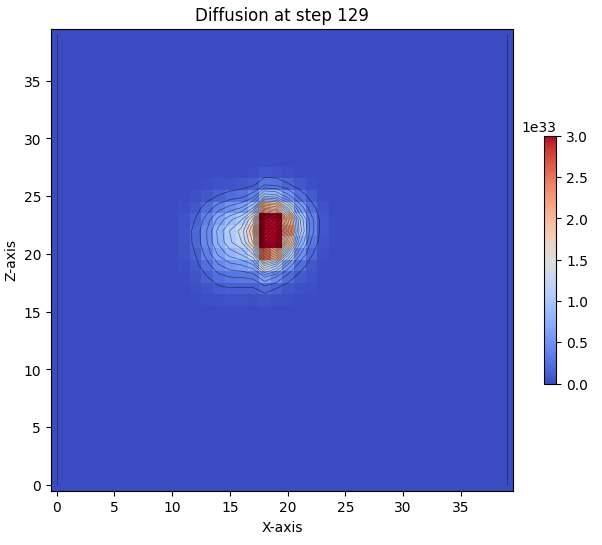
\includegraphics[width=0.22\linewidth]{Images/Cylinder-Prism-Close-2.png}
            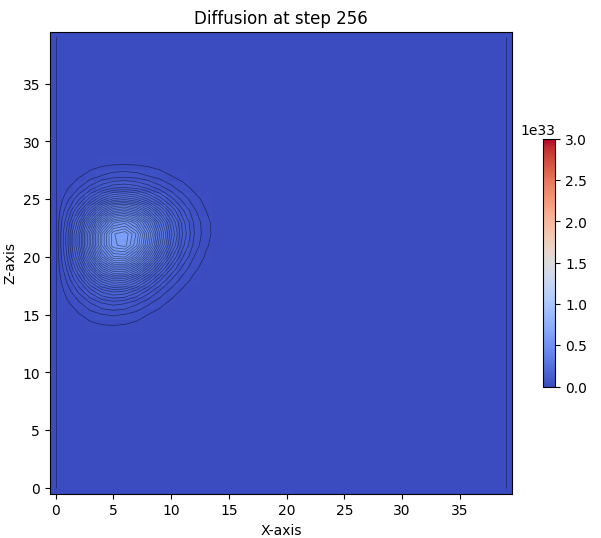
\includegraphics[width=0.22\linewidth]{Images/Cylinder-Prism-Far-3.png}
            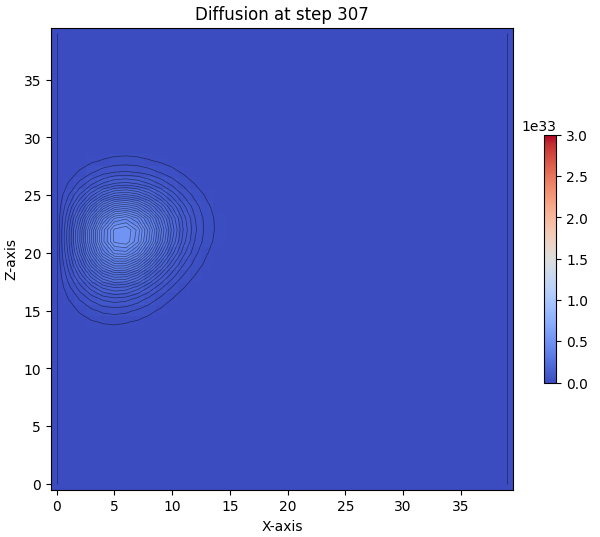
\includegraphics[width=0.22\linewidth]{Images/Cylinder-Prism-Far-4.png}\\
            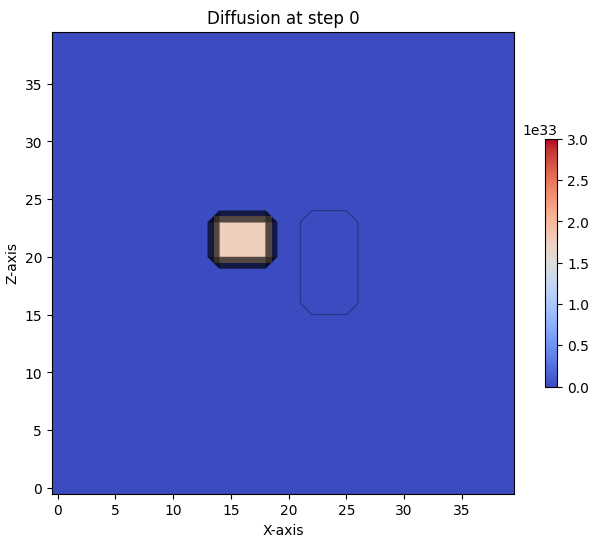
\includegraphics[width=0.22\linewidth]{Images/Cylinder-Prism-Close-1.png}
            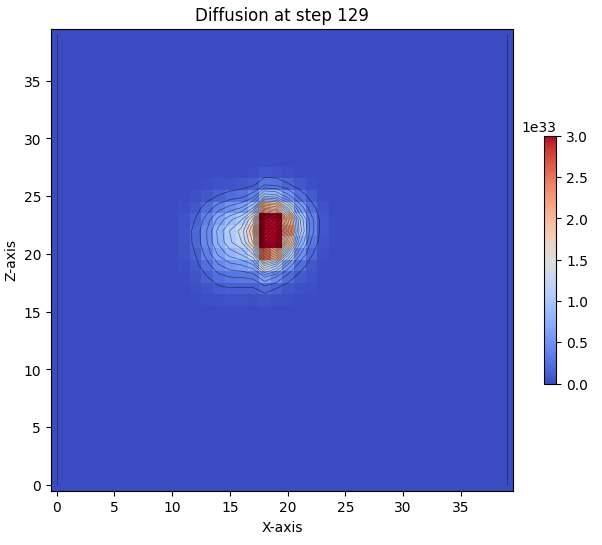
\includegraphics[width=0.22\linewidth]{Images/Cylinder-Prism-Close-2.png}
            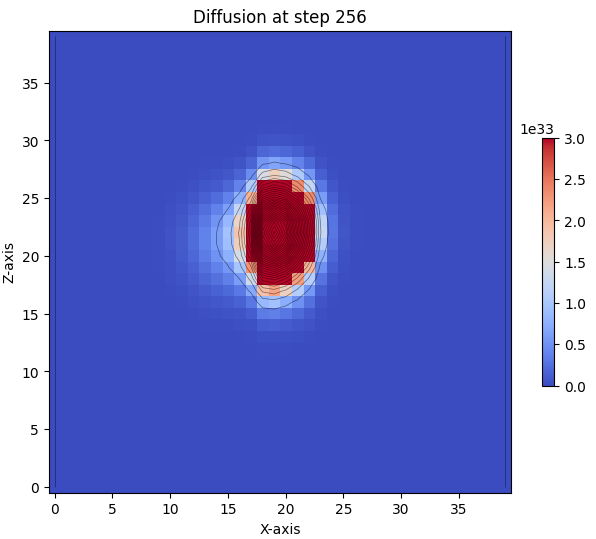
\includegraphics[width=0.22\linewidth]{Images/Cylinder-Prism-Close-3.png}
            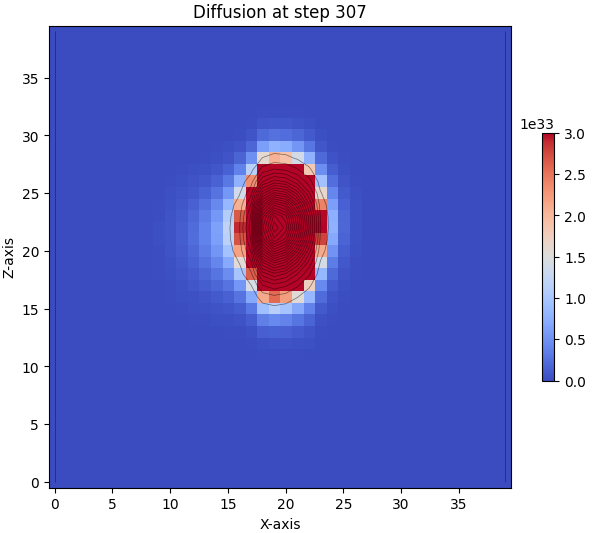
\includegraphics[width=0.22\linewidth]{Images/Cylinder-Prism-Close-4.png}
            \caption{Image of spatial distribution of neutron density for the Triangular Prism and Cylinder shaped rods. The distribution of neutron density for the 25m separation (Top) and the distribution of neutron density for the 5m separation (below)}
            \label{img:Prism-and-Cylinder-Images}
         \end{figure}

         Starting with a further separation distance of 30m between the objects, we can see from figure \ref{img:Prism-and-Cylinder-density} that the fuel rods are exhibiting a decay. The neutrons are being absorbed on the boundaries and the system is losing energy. This is shown graphically in the spatial plots of neutron density shown in \ref{img:Prism-and-Cylinder-Images}. Bringing the fuel rods closer together to a separation distance of 10m we can see that the reaction goes super-critical very quickly, and referring to equation \eqref{eq:Energy} once more, we see that $1.35 \times 10^{17}$ J of energy are released. This is equivalent to $32.3$ million tons of TNT, or about the same size as 2 detonations of \textit{Castle Bravo}, the largest nuclear test ever conducted by the United States. Castle Bravo was a thermonuclear bomb, and not a fission bomb, but due to the scale of our simulation, it makes a good comparison. Images from Castle Bravo can be seen in figure \ref{Castle-Bravo}.\\

         Now lets compare this to the energy output of the Cubes of Uranium that collide in figure \ref{URANIUM-EXPLOSION-GRID}. Looking at the density of neutrons before, we can see that the cubes exhibit an exponential decay, but as the rods are brought closer together to a separation of 10m, the reaction quickly becomes more violent than any weapon ever produced \ref{URANIUM-GRAPH-DENSITY}. This can be shown visually in the spatial distribution graphs shown in figure \ref{BOOM-BOOM-GRAPH}, as well as with the calculation of its energy release. When the fuel rods are brought close together, the energy released in the fission reaction is $3.24 \times 10^{19}$ J. To put this into perspective, this is equivalent to 7.7 billion tons of TNT. This is approximately 7700 Mega Tons of TNT, or  152 TSAR Bomba's detonating at once. This is an unfathomable amount of energy. \\

         We can say safely that the Cube approach definitely yields the highest energy output. Thinking about this mathemtically, we know that the largest surface area that can be constructed on a flat surface given an amount of material is always a square. Thus, the largest possible area to be constructed should allow for the largest amount of flux to leave the surface and travel towards the other diffusing neutrons from the opposing cube. Having the greatest possible amount of diffusable material to react, leads to the largest amount of energy consumption.\\

         You may be wondering why I didn't use Plutonium-239 for this section of the report. The simple answer is that our numbers are already very large, and the system requires very large fuel rods, so including plutonium would make the answer large enough that there wouldn't really be anything to compare it to, other than maybe the asteroid that killed off the dinosaurs 66 million years ago. \footnote{I did however calculate this for fun with the program I wrote. The asteroid that killed the dinosaurs is estimated to be equal to roughly 100 million megatons of TNT. The Plutonium Cube bomb I have constructed would be 10,000 times larger! This is enough to probably destroy the Earth.}


         \begin{figure}
            \centering
            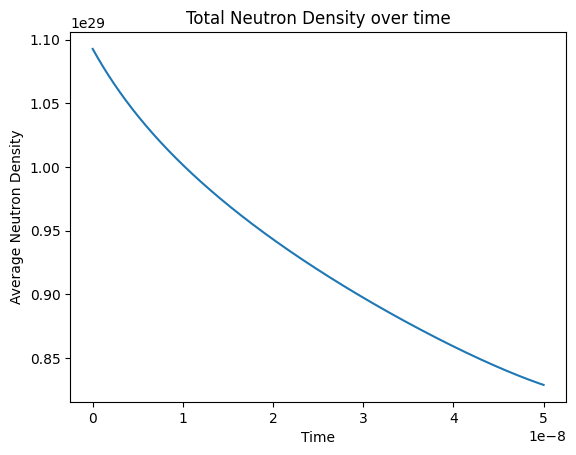
\includegraphics[width=0.4\linewidth]{Graphs/URANIUM-DECAY-GRAPH.png}
            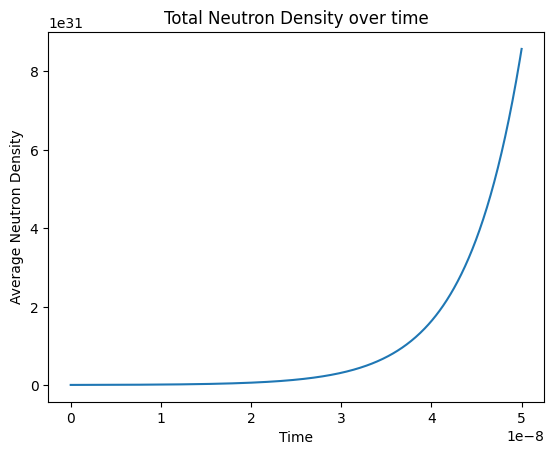
\includegraphics[width=0.4\linewidth]{Graphs/URANIUM-GROWTH-GRAPH.png}
            \caption{Image of neutron density over time for the colliding cubes of Plutonium-239.}
            \label{URANIUM-GRAPH-DENSITY}
         \end{figure}

         \begin{figure}[h!]
            \centering
            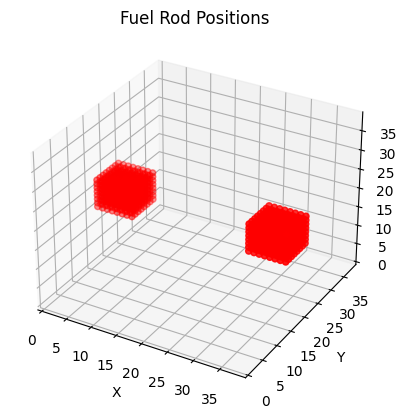
\includegraphics[width=0.3\linewidth]{Graphs/Graph_FuelRodsInGrid.png}
            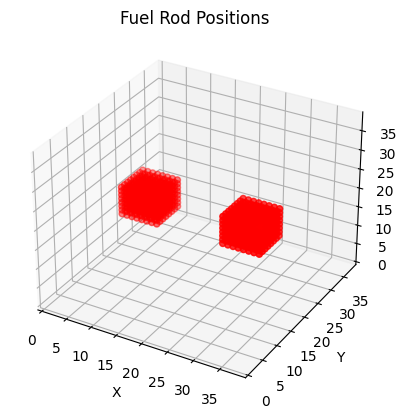
\includegraphics[width=0.3\linewidth]{Graphs/Graph_FuelRodInGrid_Middle.png}
            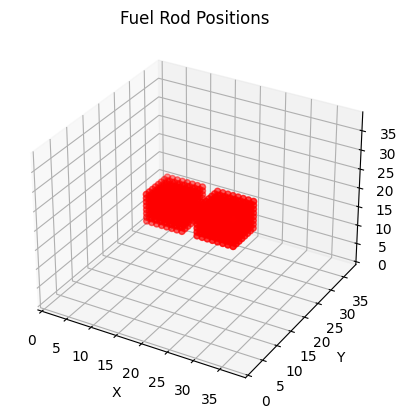
\includegraphics[width=0.3\linewidth]{Graphs/GraphFuelRodInGrid_Close.png}
            \caption{Images of the Plutonium-239 fuel rods moving closer together in the simulation grid}
            \label{URANIUM-EXPLOSION-GRID}
         \end{figure}

         \begin{figure}
            \centering
            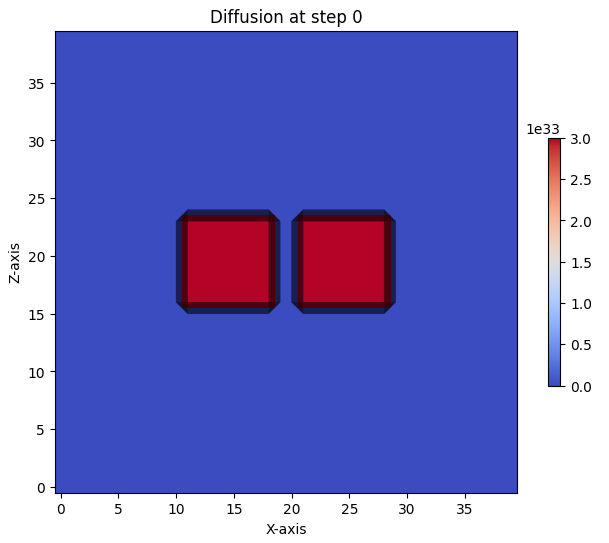
\includegraphics[width=0.22\linewidth]{Images/BOOM-BOOM-1.png}
            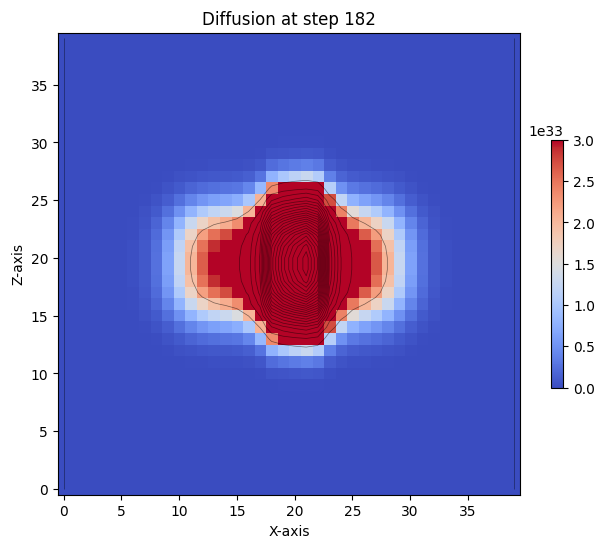
\includegraphics[width=0.22\linewidth]{Images/BOOM-BOOM-2.png}
            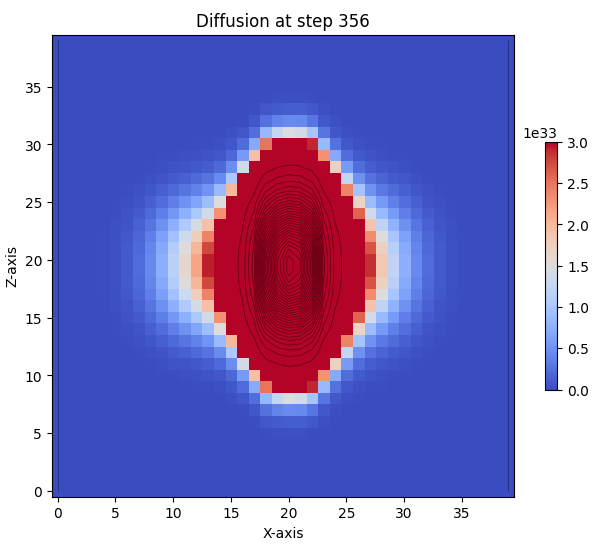
\includegraphics[width=0.22\linewidth]{Images/BOOM-BOOM-3.png}
            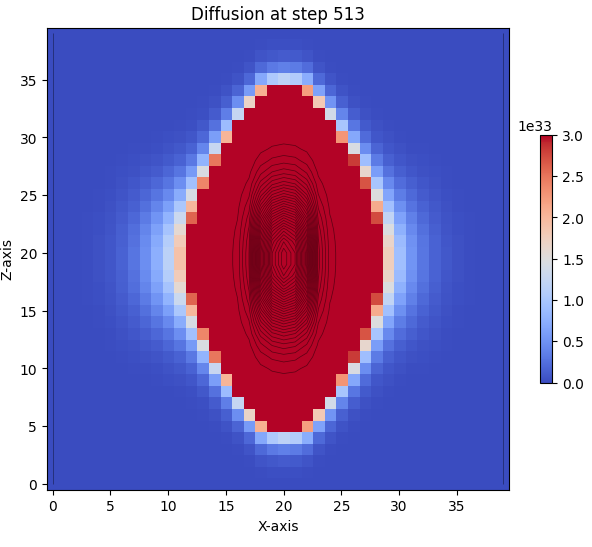
\includegraphics[width=0.22\linewidth]{Images/BOOM-BOOM-4.png}
            \caption{Image of spatial distribution of neutron density for the Plutonium-239 Cubes.}
            \label{BOOM-BOOM-GRAPH}
         \end{figure}

         \begin{figure}[t!]
            \centering
            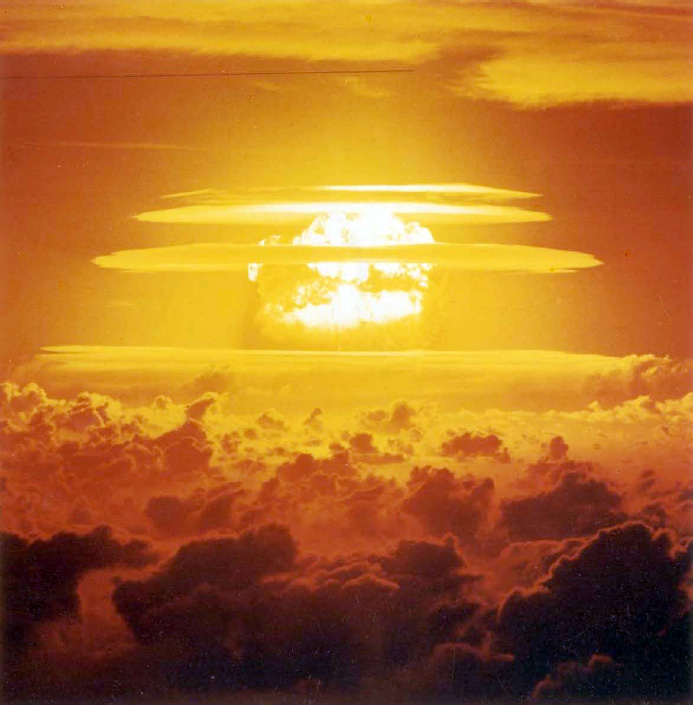
\includegraphics[width=0.24\linewidth]{Images/Castle Bravo.jpg}
            \includegraphics[width=0.336\linewidth]{Images/Castle-Bravo-Bomb.jpg}
            \caption{Images of the Castle Bravo Bomb. Castle Bravo was detonated on March 1st 1954 in Bikini Atoll. The device nuclear device is depicted on the right.}
            \label{Castle-Bravo}
         \end{figure}
   
      \subsection{Decaying, stable, and exponential neutron release}
         So far, I have shown that as the fuel rods get closer together, they eventually reach a point where the regions of interfereing flux make the production of neutrons an exponential growth instead of decay. I have also shown the minimum size the fuel rods can be in order to produce meaningful amounts of energy is about 10mm. In this section I will investigate where exactly the growth rate flips from a decay into a growth for both he Uranium-235 case with Dirichlet boundaries, and the Plutonium Case with Dirichlet boundaries. Dirichlet boundaries are being considered here instead of Neumann boundaries since we only really care about the neutrons interacting in the center of the grid, and keeping the neutrons on the boundaries just increases the density of neutrons everywhere making it harder to analyze the criticality condition.\\

         Starting in a region between a separation distance of 20 and 30, we can move the blocks slightly farther and farther away from one another until we no longer go critical. This will give us a close approximation of how far apart they need to be.

         \begin{figure}[h!]
            \centering
            \includegraphics[width=0.3\linewidth]{Graphs/Criticality-Test-U235-25m.png}
            \includegraphics[width=0.3\linewidth]{Graphs/Criticality-Test-U235-27m.png}
            \includegraphics[width=0.3\linewidth]{Graphs/Criticality-Test-U235-28m.png}
            \caption{Images of the neutron density over time for Uranium$^{235}$ cubic fuel rods at separation distances of 25m (Left), 27m (Center), and 28m (Right)}
            \label{img:Uranium-Criticality-Test}
         \end{figure}

         We can see in figure \ref{img:Uranium-Criticality-Test} that the stability condition for these $8m^3$ fuel rods is a separation distance between 27m and 28m. This might seem surprising since that is a large distance, but considering that two $8m^3$ fuel rods of Uranium is probably unstable on its own, and would weigh more than 20,000 tons, the separation distance is fairly reasonable.\\

         \begin{figure}[h!]
            \centering
            \includegraphics[width=0.45\linewidth]{Graphs/Criticality-Test-Pu-239-31m.png}
            \includegraphics[width=0.45\linewidth]{Graphs/Criticality-Test-Pu-239-36m.png}
            \caption{Images of the neutron density over time for Plutonium$^{239}$ cubic fuel rods at separation distances of 31m (Left) and 36m (Right)}
            \label{img:Plutonium-Criticality-Test}
         \end{figure}

         Since Plutonium has a higher reaction rate and diffusion constant than the Uranium (U$^{235}$ has a reaction rate of $\eta = 1.896 \times 10^8$ and a diffusion constant of $D = 2.34 \times 10^5$  vs. Pu$^{239}$ has a reaction rate of $\eta = 3.0055 \times 10^{8}$ and a diffusion constant of $D = 2.6786 \times 10^5$), we can expect that the Plutonium needs to be stored farther away than that of the Uranium. A higher diffusion constant means more neutrons are leaving the material, and at a faster rate every second, and a higher reaction rate means those neutrons are producing more neutrons in the reaction, faster.\\

         As seen in figure \ref{img:Plutonium-Criticality-Test}, the fuel rods do in fact need to be stored further away than the Uranium rods. In order to calculate this simulation, the size of the simulation grid had to be expanded to more than 40 meters. It was found during this simulation that the minimum distance that the fuel rods could be separated without causes an explosion was at 36m.


      \subsection{Dirichlet vs. Neumann boundary conditions}
         In this section we aim to compare how the different boundary conditions can affect the system's behaviour. The main difference here is the Neumann boundary conditions act as a reflector on the boundary, and reflect the neutrons back into the system. Dirichlet boundarys act as absorbing boundary conditions which remove the neutrons from the system entirely. It is defined with the following mathematical relation:

         \begin{equation}
            \phi = \alpha
         \end{equation}
      
         Where $\alpha$ is some constant value. In our case, $\alpha = 0$, and our boundary is perfectly absorbing.
         This affects the design of our nuclear device. The simulations utilizing Dirichlet conditions assume that the neutrons that diffuse away from the fuel rods leave the system, while the Neumann conditions are set up so that our device reflects the neutrons back towards the detonation center. We can predict that the Neumann conditions should lead to a more violent explosion and release of energy since there will be more lingering neutrons in the system to interact with one another during the detonation. The Neumann boundary conditions are defined as follows:
         \begin{equation}
            \frac{\partial \phi}{\partial \hat{n}} = 0 
         \end{equation}

         where $\phi$ is the neutron density, and $\hat{n}$ is the normal vector to the boundary surface.\\

         To test this I will simulate two colliding cubes of Uranium$^{235}$, and analyze how the energy output of the system changes based on the boundary conditions used. I will start with the Dirichlet case depicted in figure \ref{img:Dirichlet_Cubes}, and then move on the the Neumann case afterwards depicted in figure \ref{img:Neumann_Cubes}.
         \begin{figure}[h!]
            \centering
            \includegraphics[width=0.3\linewidth]{Graphs/Graph_FuelRodsInGrid.png}
            \includegraphics[width=0.3\linewidth]{Graphs/Graph_FuelRodInGrid_Middle.png}
            \includegraphics[width=0.3\linewidth]{Graphs/GraphFuelRodInGrid_Close.png}
            \caption{Images of the Uranium-235 fuel rods moving closer together in the simulation grid}
            \label{img:CubesInGrid}
         \end{figure}

         \begin{figure}[t]
            \centering
            \includegraphics[width=0.32\linewidth]{Graphs/DirichletCubes_Density_Vs_Time_Far.png}
            \includegraphics[width=0.32\linewidth]{Graphs/DirichletCubes_Density_Vs_Time_Middle.png}
            \includegraphics[width=0.32\linewidth]{Graphs/DirichletCubes_Density_Vs_Time_Close.png}
            \caption{Average neutron density over time for the Dirichlet Boundary Conditions at a separation distance of 25m, 20m, and 10m}
            \label{img:Dirichlet_Cubes}
         \end{figure}

         \begin{figure}[t]
            \centering
            \includegraphics[width=0.25\linewidth]{Images/Dirichlet-25m-Image.png}
            \includegraphics[width=0.25\linewidth]{Images/Dirichlet-20m-Image.png}
            \includegraphics[width=0.25\linewidth]{Images/Dirichlet-10m-Image.png} \\
            \includegraphics[width=0.25\linewidth]{Images/Neumann-25m-Image.png}
            \includegraphics[width=0.25\linewidth]{Images/Neumann-20m-Image.png}
            \includegraphics[width=0.25\linewidth]{Images/Neumann-10m-Image.png}
            \caption{Neutron density heat map for Dirichlet boundary conditions (Top), and Neumann boundary conditions (Bottom), for distances of 25m, 20m, and 10m separation respectively.}
            \label{img:Boundary-Condition-Testing}
         \end{figure}

         As shown in figure \ref{img:Boundary-Condition-Testing}, we still get a similar explosion in the center, but the values around the edges of the simulation are much greater! We can conclude here that the effect only really makes a difference in neutron density when the objects are closer to the boundaries and farther away. This is likely because the reaction is strong enough at the center that the production of neutrons overpowers the absorbing or reflecting boundary conditions. \\

         The most important thing to notice however is that the Neumann boundary conditions require the objects to be farther apart. Since the average density in the simulation grid is higher even at farther separation distances, the chance of an explosion is very high. We can conclude that Dirichlet boundary conditions should be used when trying to keep a stable reaction (at $k = 1$ for example) where the fuel rods are either slowly decaying, or equally producing neutrons and losing them. Neumann boundary conditions should be used in the design of something like a nuclear weapon, since more neutrons are staying in the simulation.

         \begin{figure}[b]
            \centering
            \includegraphics[width=0.32\linewidth]{Graphs/NeumannCubes_Density_Vs_Time_Far.png}
            \includegraphics[width=0.32\linewidth]{Graphs/NeumannCubes_Density_Vs_Time_Middle.png}
            \includegraphics[width=0.32\linewidth]{Graphs/NeumannCubes_Density_Vs_Time_Close.png}
            \caption{Average neutron density over time for the Neumann Boundary Conditions at a separation distance of 25m, 20m, and 10m}
            \label{img:Neumann_Cubes}
         \end{figure}

    \section{  Methods}
      In order to simulate the neutron diffusion process for various materials and shapes I used a 6 point stencil in 3D space to calculate the Laplacian using a finite difference method. The method was adapted from the \textit{diffusion-2d} method developed in class. In order to determine the appropriate time step size to ensure numerical stability, I implemented a CFL condition dependant on the grid spacing and diffusion constant. The Satisfied CFL condition is written mathematically below:
      
      \begin{equation}
         \delta t \le \frac{\delta x^2}{6D}
      \end{equation}

      This ensures numerical stability and helps prevent the solution from diverging. For safety, I set my timestep to be a quarter of this value, so I was sufficiently far from breaking the condition. The numerical stability in this simulation is particularly important, since the program implentation deals with numbers that are both extremely large (neutron density per cubic meter) and extremely small (timestep in nanoseconds). The machine precision of floating point numbers in python by default is
      roughly 17 digits \cite{Python-Floating-Point-Error}, so we need to be careful that our small timesteps and large densities don't cause a propagation of error from the floating point precision. Since our implentation needs to loop over 3-spatial and 1 temporal dimension, the number of iterations can also propagate the error. Ensuring that our finite difference method has as little error as possible was of key importance. The diffusion-3d implentation has an error propagation of $\mathcal{O} (\delta t + \delta x^2)$.\\

   \section{   Discussion and Ideas for Extension}

      There are a few key points that need to be discussed about the implementation, as well as two future extensions to the project which may help make the simulation more accurate. The first hurdle I had to deal with when designing the diffusion reaction was the fuel rods themselves. The fuel rods are initialized as a class and and then inserted into the simulation grid. But the simulation grid does not know which fuel rod is which, it only knows that there are now source terms present in its initial conditions before it begins to be diffused. When the objects are placed into the grid, the grid sees them as hundreds of tiny fuel sources that are located as close together as possible in the grid. When the diffusion occurs, the program sees that two sources that each produce neutrons are close together, so the flux between them is high, and declares that the system should explode. This means that the individual fuel rods would blow up immediately when the first timestep occurs, regardless of separation between the two fuel rods, regardless of shape, and regardless of size and density. To fix this, I needed to find a way to diffuse the neutrons, but only have the neutrons react if they came from opposing fuel rods within the grid. To do this, I took a slice of the grid near the center where the neutrons from both sources would initially meet eachother for the first time, and allowed the neutrons within that region to react. This ensures that the point sources that make up the fuel rods will not cause the system to explode. However, this implementation does not account for the fact that neutrons in the same central region of the grid that are from the same fuel source can now multiply with eachother. While there is nothing stopping this from happening in reality, it happens much more throughout the simulation than is physically reasonable. An implementation to try in the future would be to make the fuel rod sources Tuples, and assign each grid point a value (density) and an identifier specifying which neutron source it was emitted from. Only neutrons with opposing identifiers or created neutrons from the reaction would be allowed to multiply. This will not be straightforward to implement however since you would then also need to keep track over every neutron in the reaction, and since there are many of them, you can run into memory issues. \\

      The second extension to this project that could help preserve more physics would be to implement a moving fuel source. Inside of an atomic bomb, the detonation and violent reaction occurs when the fuel rods are smashed together. To simulate this in my project, I simulated the diffusion at each spatial distance until the rods were colliding together to give a picture of how it would behave. This however does not account for the fact that the neutrons emitted from the fuel sources would leave a streak or comet trail behind the objects as the move together, and slightly changes the density distribution in the diffusion reaction process. To fix this, I will implement a vector field containing vector data for the fuel rods, and set them to move closer together until they have collided. This would require implementing a \textit{Material Derivative} instead of a \textit{Diffusion Reaction} equation, which behaves similarly but has an additional velocity term. This would be difficult to implement since it would require another 3D array in memory which contains the vector information at each point in the grid, and would be updated at each timestep. It would also require collision detection between the two fuel rod sources, and the complexity of such a simulation has been discussed to be outside the scope of this course. \\

      Both extensions to the project would require additional memory management, and would reduce the simulation time of the program, but have the possibility of adding more physical realism to the simulation. 

   \section{   Conclusion}
      To conclude, this project successfully analyzes the process of neutron diffusion and reaction inside of a reaction chamber, implementing the neutron-reaction equation in python using a 3D stencil and a finite difference method. I found that materials such as U$^{235}$ and Pu$^{239}$ are strong fissile source materials for the reaction. Plutonium-239 in particular yields the highest rate of diffusion combined with the highest reaction rate of fissile neutrons, but Uranium-235 is a strong candidate, being more useful due to its ease of access of material compared to Plutonium. I also showed how elements such as Iron or Americium are poor candidates to use for fuel sources, since they have higher absorption rates than fission rates for their emitted neutrons \ref{Americium}, or require too much energy to begin the process for too little of a yield ($D_{\text{Fe}} = 0.0024 m^2/s$) \cite{article}. I determined that the optimal shape for the highest energy output of the system were cubes, which had the capacity to create an explosion more than 152 times the energy output of the TSAR-Bomba. Investigating the smaller scale fuel rod sources of sizes around 1 millimeter to 1 centimeter, we found that the energy available from fission is negligible at 1mm, but quickly scales up to the size of a small explosion by the time the size reaches 1cm.

    
   \newpage
   \pagenumbering{arabic}
   \vspace{-0.5cm}
   \bibliographystyle{ieeetr}
   \bibliography{report-citations}
\end{document}
